% Unofficial UChicago CS Poster Template
% v1.1.0 released September 8, 2022
% https://github.com/k4rtik/uchicago-poster
% a fork of https://github.com/anishathalye/gemini

\documentclass[final]{beamer}

% ====================
% Packages
% ====================

\usepackage[T1]{fontenc}
\usepackage{lmodern}
\usepackage[size=custom,width=120,height=72,scale=1.0]{beamerposter}
\usetheme{gemini}
\usecolortheme{uchicago}
\usepackage{graphicx}
\usepackage{booktabs}
\usepackage{doi}
\usepackage[numbers]{natbib}
\usepackage[patch=none]{microtype}
\usepackage{tikz}
\usepackage{pgfplots}
\pgfplotsset{compat=1.18}
\usepackage{anyfontsize}

\pdfstringdefDisableCommands{%
\def\translate#1{#1}%
}

% ====================
% Lengths
% ====================

% If you have N columns, choose \sepwidth and \colwidth such that
% (N+1)*\sepwidth + N*\colwidth = \paperwidth
\newlength{\sepwidth}
\newlength{\colwidth}
\setlength{\sepwidth}{0.025\paperwidth}
\setlength{\colwidth}{0.3\paperwidth}

\newcommand{\separatorcolumn}{\begin{column}{\sepwidth}\end{column}}

% ====================
% Title
% ====================

\title{Elucidation of the mechanism of a Morita-Baylis-Hillman type reaction catalyzed by engineered enzymes using transition path sampling}

\author{Sree Ganesh Balasubramani \inst{1} \and Steven Schwartz \inst{1} }

\institute[shortinst]{\inst{1} Department of Chemistry and Biochemistry, The University of Arizona}

% ====================
% Footer (optional)
% ====================

\footercontent{
  \href{https://www.example.com}{https://sreeganb.github.io} \hfill
  %ABC Conference 2025, New York --- XYZ-1234 
  \hfill
  \href{mailto:sreegb@arizona.edu}{sreegb@arizona.edu}}
% (can be left out to remove footer)

% ====================
% Logo (optional)
% ====================

% use this to include logos on the left and/or right side of the header:
% \logoright{\includegraphics[height=7cm]{logo1.pdf}}
% \logoleft{\includegraphics[height=7cm]{logo2.pdf}}

% ====================
% Body
% ====================

\begin{document}
\addtobeamertemplate{headline}{}
{
    \begin{tikzpicture}[remember picture,overlay]
      \node [anchor=north west, inner sep=3cm] at ([xshift=0.0cm,yshift=-2.4cm]current page.north west)
      {
\includegraphics[height=5.0cm]{logos/ua_stack_rgb_4.eps}}; % also try shield-white.eps
      %\node [anchor=north east, inner sep=3cm] at ([xshift=0.0cm,yshift=2.5cm]current page.north east)
      %{\includegraphics[height=8.0cm]{logos/cs-logo-white.png}};
    \end{tikzpicture}
}

\begin{frame}[t]
\begin{columns}[t]
\separatorcolumn

\begin{column}{\colwidth}

  \begin{block}{Introduction to TPS}

    Some block contents, followed by a diagram, followed by a dummy paragraph.

   % \begin{figure}
   %   \centering
   %   \begin{tikzpicture}[scale=6]
   %     \draw[step=0.25cm,color=gray] (-1,-1) grid (1,1);
   %     \draw (1,0) -- (0.2,0.2) -- (0,1) -- (-0.2,0.2) -- (-1,0)
   %       -- (-0.2,-0.2) -- (0,-1) -- (0.2,-0.2) -- cycle;
   %   \end{tikzpicture}
   %   \caption{A figure caption.}
   % \end{figure}

    

  \end{block}

  \begin{block}{Directed evolution and the design of enzymes}

    \begin{itemize}
      \item Is it possible to design enzymes that perform complicated reactions such as this easily?
      \item Elucidate the mechanism of the double proton transfer reaction 
      \item Find the transition state and propose mutations that improve the catalytic efficiency
    \end{itemize}

  \end{block}

  \begin{block}{A highlighted block}
    \begin{figure}
        \centering
        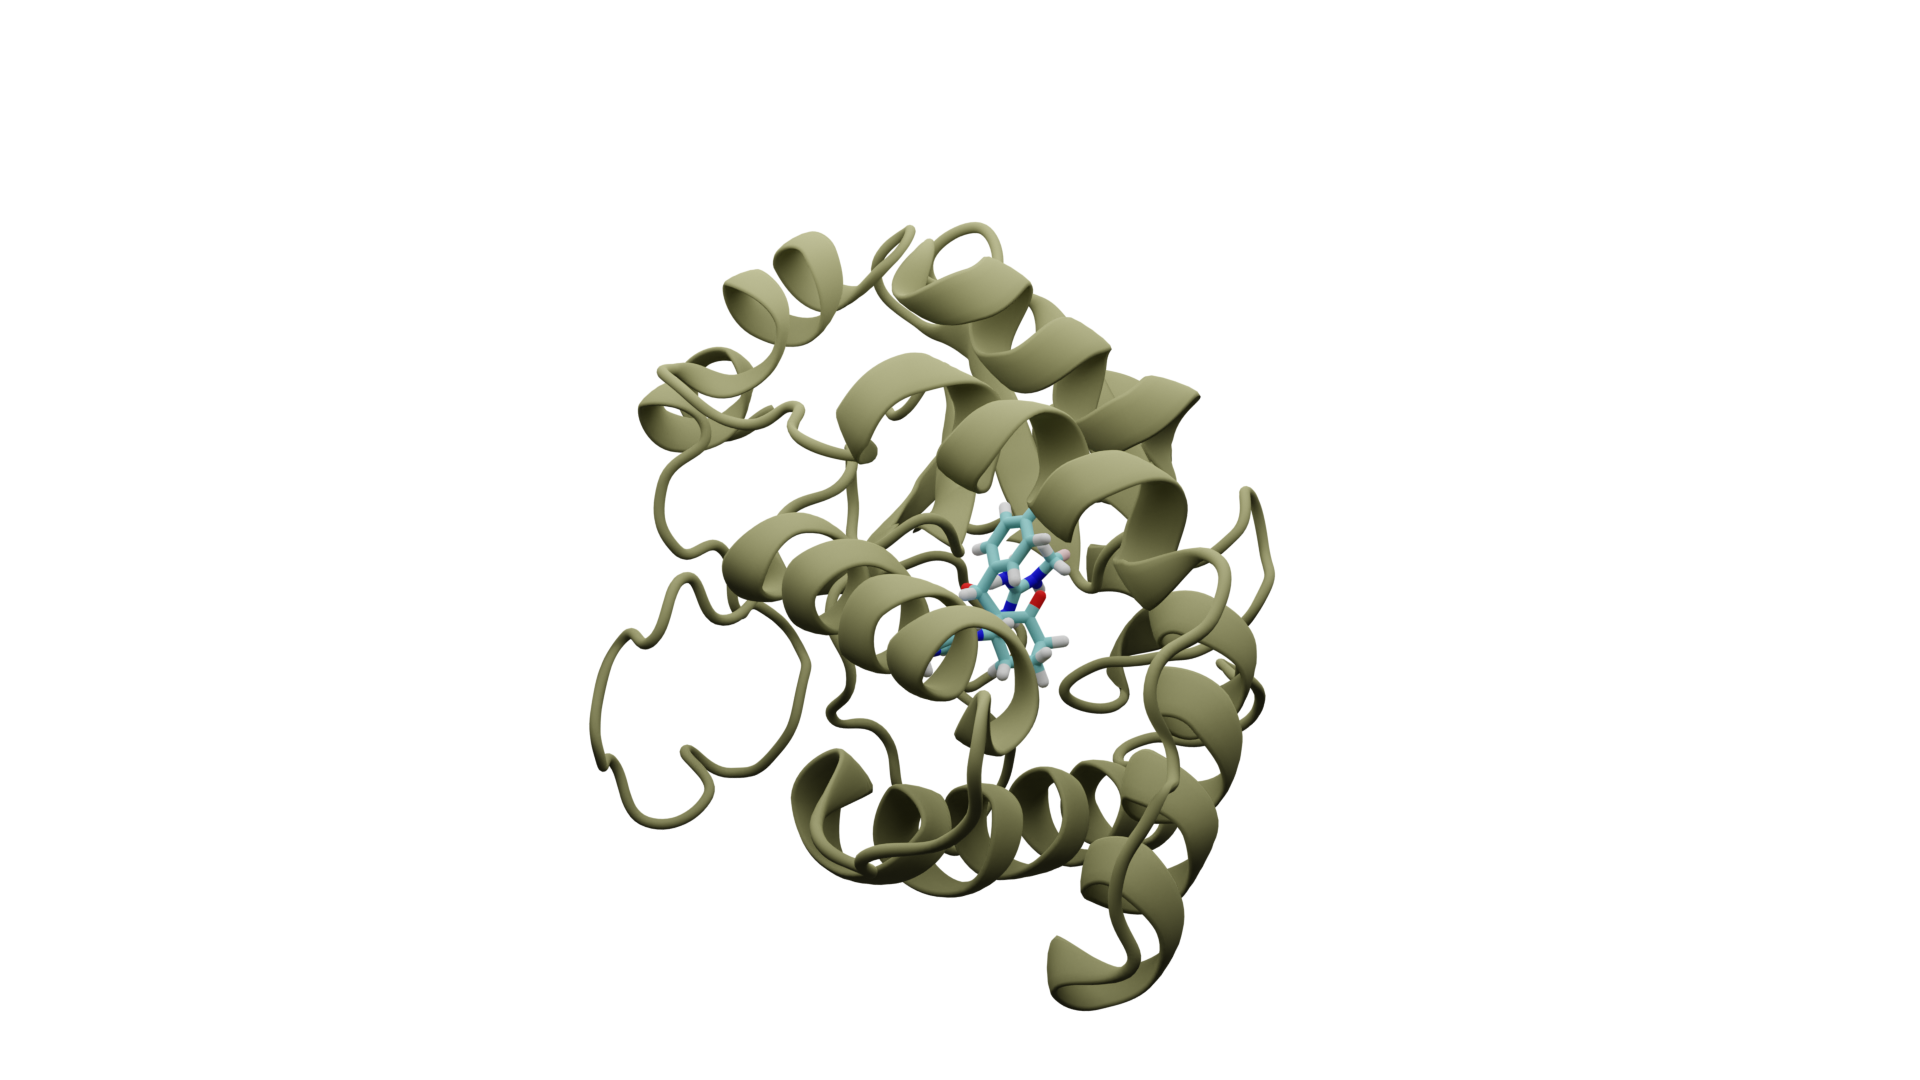
\includegraphics[scale=0.5]{figures/reac-121.png}
        \caption{The protein witht he substrates bound}
    \end{figure}

  \end{block}

\end{column}

\separatorcolumn

\begin{column}{\colwidth}

  \begin{block}{A block containing an enumerated list}

    
  \end{block}

  \begin{block}{Fusce aliquam magna velit}

    %   \begin{figure}
    %  \centering
    %  \begin{tikzpicture}
    %    \begin{axis}[
    %        scale only axis,
    %        no markers,
    %        domain=0:2*pi,
    %        samples=100,
    %        axis lines=center,
    %        axis line style={-},
    %        ticks=none]
    %      \addplot[red] {sin(deg(x))};
    %      \addplot[blue] {cos(deg(x))};
    %    \end{axis}
    %  \end{tikzpicture}
    %  \caption{Another figure caption.}
    %\end{figure}

  \end{block}

  \begin{block}{Nam cursus consequat egestas}

  \end{block}

\end{column}

\separatorcolumn

\begin{column}{\colwidth}

  \begin{exampleblock}{A highlighted block containing some math}

    
    %\heading{A heading inside a block}

    

    %\heading{Another heading inside a block}

    

  \end{exampleblock}

  \begin{block}{Nullam vel erat at velit convallis laoreet}

    

    %\begin{table}
    %  \centering
    %  \begin{tabular}{l r r c}
    %    \toprule
    %    \textbf{First column} & \textbf{Second column} & \textbf{Third column} & \textbf{Fourth} \\
    %    \midrule
    %    Foo & 13.37 & 384,394 & $\alpha$ \\
    %    Bar & 2.17 & 1,392 & $\beta$ \\
    %    Baz & 3.14 & 83,742 & $\delta$ \\
    %    Qux & 7.59 & 974 & $\gamma$ \\
    %    \bottomrule
    %  \end{tabular}
    %  \caption{A table caption.}
    %\end{table}

    

  \end{block}

  \begin{block}{References}

    \nocite{*}
    \footnotesize{\bibliographystyle{plainnat}\bibliography{poster}}

  \end{block}

\end{column}

\separatorcolumn
\end{columns}
\end{frame}

\end{document}
